
\section{Measuring subjective versus objective risks}

\subsection{Proxy of objective job risks using real-time machine-learning}

In the previous section, we directly compare perceived risks with the ex-post realization of job transitions. We reject the perfect foresight assumption, as ex-ante perceived risks differ from realized job flow rates. However, this gap cannot be fully interpreted as a deviation from a full-information-rational-expectations benchmark from an ex-ante point of view. Even if perceived job risks are fully rational ex-ante, conditional on real-time economic conditions, newly realized shocks due to changes in the macroeconomy may still induce a gap between them. We would need a proxy for true ex-ante job risks to characterize the deviations of perceived job risks from a FIRE benchmark.

We adopt the methodology of \cite{bianchi2022belief} to use machine-learning efficient forecasts of labor market transition rates to proxy the true ex-ante job transition risks. Specifically, for each month $t$ in our historical sample, we use a Lasso model to select the set of variables that makes the best in-sample prediction of realized flow rates over a 10-year window up to $t$, as defined in Equation \ref{eq:lasso}. Note that the coefficients are time-specific due to the real-time nature of this estimation procedure, i.e., the prediction model is estimated using only historical information up to time $t$. 
\begin{equation}
\begin{split}
\label{eq:lasso}
%    & {JF}_{t,t+3} = \Gamma^t X_{t} + \epsilon_{t} \\
%&    \widehat{JF}^*_{t+3|t}=\widehat \Gamma^{t*}X^*_t
 &   JF_{t+3|t} = \beta_0^t + \sum_{i=1}^{p} \beta_i^t X_{t,i} + \epsilon_t, \\
 &   \text{subject to} \quad \sum_{i=1}^{p} |\beta_i^t| \leq \lambda.
\end{split}
\end{equation}

Next, we generate a 3-month-ahead out-of-sample predicted value, $\widehat{\text{JF}}^*_{t+3|t}$, based on the optimally chosen coefficient estimates, $\beta^{t*}$, obtained through k-fold cross-validation. (Equation \ref{eq:lasso_prediction})
\begin{equation}
    \label{eq:lasso_prediction}
    \widehat{JF}^*_{t+3|t} =  \beta_0^{*t} + \sum_{i=1}^{p} \beta_i^{*t} X_{t,i}
\end{equation}

Approximately 600 time series are considered as candidate predictors of job flow rates. They include not only real-time macroeconomic variables but also forward-looking expectations of households and professional forecasts. Specifically, the following categories of predictors are included:
\begin{itemize}
    \item Real-time macroeconomic data, such as inflation, unemployment rate, GDP growth, etc. We ensure that these series are real-time data rather than retrospectively revised figures.
    \item Household expectations from the Michigan Survey of Consumers (MSC).\footnote{Codebook: \url{https://data.sca.isr.umich.edu/subset/codebook.php}.} We use disaggregated indices instead of composite indices in the survey. These indices contain rich information on how average households perceive the macroeconomy and their personal finances. Notably, we include survey questions that elicit respondents' recent exposure to macroeconomic news, their intentions to purchase durable goods, and the reasoning behind their reported expectations (e.g., ``it is not a good time to buy a car because the price is too high.'').\footnote{Survey questions that ask about not only ``what'' but also ``why'' contain useful information in understanding household expectations \citep{colarieti2024and,haaland2024measuring}.} 
    \item Realized job-finding and separation rates calculated from the Current Population Survey (CPS) \citep{fujita2009cyclicality}. Given the persistence of flow rates, recent job flow realizations may serve as strong predictors of future transitions.  %\item Real-time newspaper topics constructed from LDA models.
    \item Consensus professional forecasts of the macroeconomy from the Survey of Professional Forecasters (SPF). Even professional forecasters have often been shown to deviate from the FIRE benchmark due to information rigidity and overreaction \citep{coibion2015information,bordalo2020overreaction,bianchi2022belief}. Nonetheless, professional forecasts' views reflect one of the most sophisticated and informed perspectives on the macroeconomy in real time. Indeed, \cite{carroll2003macroeconomic} treats professional forecasts as a proxy for real-time rational forecasts. Here, however, we do not make such an assumption, instead recognizing their potential, as part of the broader real-time information set.
 \end{itemize}

In theory, there is no restriction to what series we can use as long as it was measured in real time and could have been, in principle, in the information set of agents making forecasts standing at $t$. In practice, we cannot exhaustively account for all potentially relevant real-time information. However, given the extensive coverage of our selected series, they collectively serve as a reasonable proxy for the hypothetical complete real-time information set.  

One particularly important input in real-time forecasting is the directly reported perceived job risks. A large body of literature has shown that individuals have advance information, or superior information, about their future job changes which economists bystanders might have otherwise attributed to unexpected shocks \citep{hendren2017knowledge}. Using average perceived risks is therefore meant to take care of this fact. If household expectations indeed predict subsequent labor market transition rates, as shown in the previous section, our machine-learning model would identify them as useful predictors. 

In practice, however, we cannot always rely on perceived risks by households, as such data have only been available in SCE since 2013. Instead, we indirectly include all time series on household expectations in MSC, assuming that perceived job risks are ultimately correlated with other household expectations. Alternatively, we also explicitly impute perceived risks using such an assumption in Section \ref{subsec:imputing}. Both approaches yield similar results.   


\paragraph{Real-time job risks.} 
The real-time machine-efficient prediction of job transition rates is plotted in Figure \ref{fig:predictive_regression} against the realized job transition rates. Each point on the real-time forecast risk line corresponds to a forecast generated using only the information up to that point in time, based on a selected set of predictors with the optimally chosen penalization to prevent overfitting. Overall, the machine-efficient forecasts predict subsequent labor market movements with high accuracy, with the notable exception of major recessions, particularly the COVID-19 crisis in the first quarter of 2020. 

This suggests that near-horizon labor market flow rates are highly predictable as long as all the relevant information is used, especially during normal times. When it comes to sudden crisis episodes such as the COVID pandemic outbreak, machine-efficient forecasts fail to anticipate the resulting labor market disruptions, consistent with the unexpected nature of such events. Nonetheless, once the initial shock unfolds, the machine-efficient forecasts are able to predict the subsequent changes in job flows with reasonable accuracy.
\begin{figure}[pt]
    \caption{Machine prediction of labor market outcomes}
    \label{fig:predictive_regression}
    \begin{center}
\adjustimage{max size={0.7\linewidth}}{text/chapter2/Figures/predicted_comparison_1step_JF_realization_real_time.pdf} \\
\vspace{0.4cm}
\adjustimage{max size={0.7\linewidth}}{text/chapter2/Figures/predicted_comparison_1step_JS_realization_real_time.pdf} 
    \end{center}
\floatfoot{\footnotesize{3-mouth-ahead job risks generated from real-time machine-learning forecasts using real-time data for each 10-year rolling window (in scale of 0-100).}}
\end{figure}

Figure \ref{fig:why_real_time} highlights the importance of using real-time forecasts without relying on hindsight. In most of the sample periods, the machine-efficient real-time forecasts of job-finding and separation rates exhibit non-zero forecast errors, implying even the rational ex-ante job risks would not have perfectly anticipated the subsequent realization of macro flow rates. In contrast, one-shot retrospective machine-learning forecasts, by which we mean the forecasts made based on the hindsight of the entire sample period, produce a forecast of job transition rates that have on average zero forecast errors. This was essentially due to overfitting to latter realizations of the history. This suggests that compared to a well-informed benchmark of ex-ante risks, unexpected shocks to realized job flow rates inevitably occur. 

\begin{figure}[!ht] \centering  % [h!]
\caption{Forecast errors of real-time versus retrospective job risks} 
\label{fig:why_real_time}
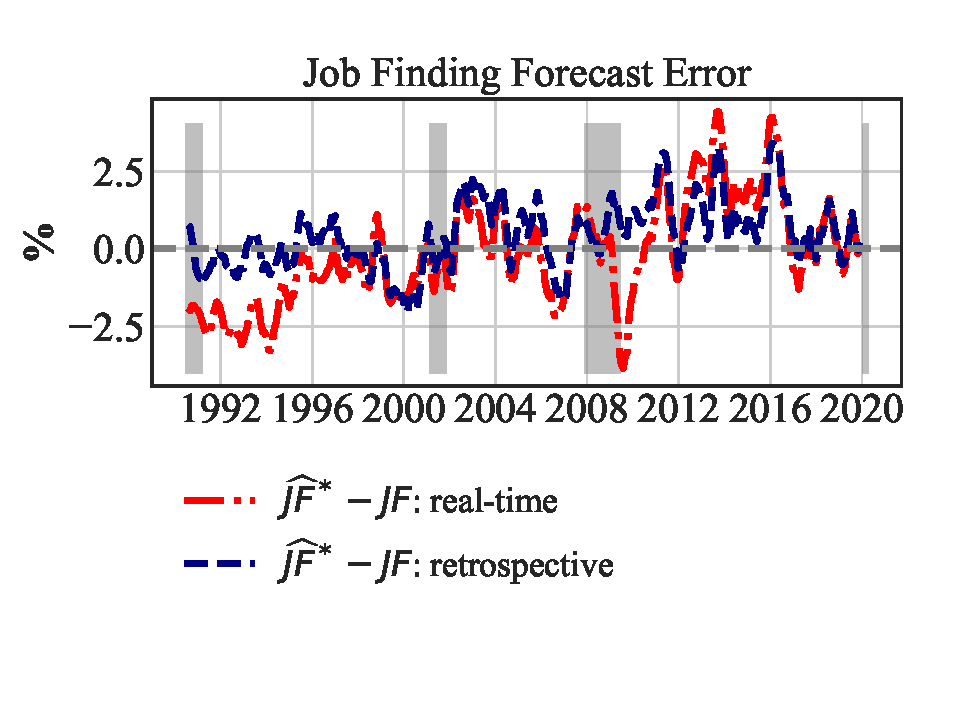
\includegraphics[width=0.49\linewidth]{text/chapter2/Figures/real_time_one_shot_comparison_1step_JF.pdf} 
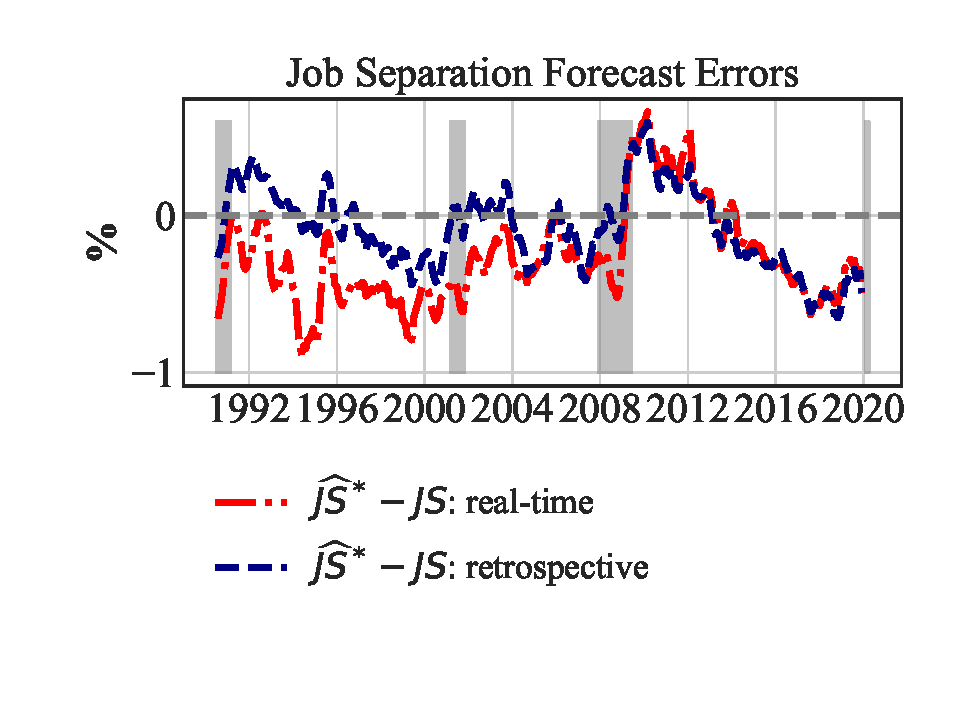
\includegraphics[width=0.49\linewidth]{text/chapter2/Figures/real_time_one_shot_comparison_1step_JS.pdf} 
\floatfoot{\footnotesize{This figure compares the forecast errors of the machine-learning predictions of job finding and separation rates generated by two different approaches: real-time versus retrospective forecasting. All rates are in the units of percent chance.}}
\end{figure}

\paragraph{What predicts labor flows?} 
One of the commonly selected predictors in real-time forecasting is the unemployment rate. A higher current unemployment rate predicts a higher separation rate and a lower job-finding rate. This is not surprising, as the unemployment rate reflects the overall state of the labor market and impacts the subsequent transition rates. 

In addition, many forward-looking variables in MSC consistently predict future labor market outcomes. The fact that many expectational variables can predict labor transitions suggests that households possess meaningful forward-looking views on job risks. It is worth noting that such predictability should not be interpreted as causal. We take it as evidence that information available ex-ante and predictable for macroeconomic outcomes is indeed incorporated into households' expectations about their future employment prospects.   

In particular, three types of household expectations commonly show up in the Lasso model selections. The first set of variables directly relates to the self-reported exposure to labor market news. In particular, we find that when households report having heard favorable (unfavorable) news about the labor market, it predicts subsequent increases (decreases) in job finding and decreases (increases) in job separation. The second group of expectational variables is broadly about future personal finance and its recent realizations. The third set of predictors that are constantly selected across real-time forecasting samples is forward-looking actions by households, the most notable of which is the durable goods purchase intentions. Several papers \citep{carroll1997unemployment,harmenberg2021consumption} have empirically established the negative relationship between job risk and the propensity to purchase durable goods, consistent with structural models predicting that costly adjustments in durable goods are highly sensitive to income uncertainty, due to both precautionary saving motives and ``wait-and-see'' mechanisms. Therefore, the correlation between intentions of future durable purchasing and subsequent labor market movements is likely driven by their respective correlation with ex-ante perceived job risks. In addition, durable goods demand plays a crucial role in aggregate fluctuations through general-equilibrium forces, as shown in \citet{mckay2021lumpy}.Interestingly, survey questions that directly elicit rationales by households on their expectations, such as ``not buying a durable due to high uncertainty'', also help predict future job transition rates. This confirms the finding by \cite{leduc2016uncertainty} also based on the uncertainty question elicited in the MSC. 

\paragraph{Comparing Machine-Learning Forecasts with Simple Time Series Models.}
Are these predictions as good as simply one univariate time series prediction? Given the persistence and time-series correlation of flow rates, the answer is not necessarily yes. We therefore compare the mean squared errors (MSE) of real-time forecasts using all datasets with a real-time forecast that is only using an AR(1) model. We show that the Lasso prediction based on a large time series dataset slightly outperforms the AR(1) model in terms of MSEs. Figure \ref{fig:real_time_ar} in the Appendix compares the risk forecast based on Lasso and AR(1). In most of the sample period, the two track each other quite well. The most noticeable divergence occurred during the pandemic where AR(1) forecast overforecast job separations due to the historical persistence of separation rate while Lasso model-based separation risk is predicted to have a more temporary reversal following the initial dramatic spike.


%XQ: I stopped here last time. 
\subsection{Backcasting perceptions: what were people thinking then?}
\label{subsec:imputing}

Directly observed perceived risks have only been available in SCE since 2013. Meanwhile, a wide range of expectations have been surveyed in MSC for a much longer time span, some of which go back to as early as the 1960s. Under the assumption that the correlations between different expectations have been stable\footnote{We reject the null hypothesis of a structural break based on the test by \citet{andrews1993tests}.}, we can utilize the estimated correlation between perceived job risks in SCE and other expectations in MSC in the overlapping sample period to impute the out-of-sample perceived risks back in earlier history. We use a Lasso model to select among many contemporaneous variables that best predict the measured perceived job risks, as specified below. 
\begin{equation}
\begin{split}
    & \widetilde{\text{JF}}_{t+3|t} = \gamma_0^t + \sum_{i=1}^{p} \gamma_i^t X_{t,i} + \epsilon_t, \\
    &  \text{subject to} \quad \sum_{i=1}^{p} |\gamma_i^t| \leq \lambda.
\end{split}
\end{equation}

where $\widetilde{JF}_t$ is the average 3-month job-finding expectations at month $t$. The regressor vector $X_t$ includes both $\text{EXP}_t$,  a vector of contemporaneous belief variables, and $\text{REAL}_t$, a vector of real-time macro aggregates. The reason why we also include real-time aggregate realizations, not just expectational variables, is that in theory, this information may have been in the information set of the agents forming expectations. We again use cross-validation to determine the optimal degree of regularization of the Lasso model and obtain the optimal model coefficients of the selected list of predictors, we denote as $\gamma^{*t}_i\forall i=1,2...p$. 

We externally validate our imputation methodology utilizing the fact that the expectations about 1-year-ahead inflation, and 5-year horizon job separation probability are measured in MSC for a much longer period. Figure \ref{fig:impute_cv_with_msc_separation_inflation} in the Appendix suggests that the imputation based on only 2013-2022 in-sample can generate out-of-sample backcasts of these two expectations that almost mimic the observed data by a correlation of 80\%-99\%. \footnote{Figure \ref{fig:impute_cv_with_msc_ue} further validates that the imputed unemployment rate expectation in SCE almost perfectly correlates with the unemployment rate expectation index in MSC, although the two are not measured in the same way. This suggests that even across the two surveys the imputation methods yield valid backcasts of beliefs.} 

%In the Appendix \ref{appendix:sensitivity_imputation}, we compare the sensitivity of the imputed series regarding the inclusion of the pandemic period, the inclusion of realized macroeconomic variables, and the use of other machine learning models. The imputed series remains very similar. 

What are the most important covariates of the perceived risks? It turns out that numerous expectation variables in MSC, such as durable purchase, news heard about economic conditions, recent experience, and future expectations of personal finance. In Figure \ref{fig:vars_rank} in the Appendix, we list the top predictors of perceived finding and separation rates, respectively. The directions of these correlations all have sensible and intuitive interpretations.  

In addition to expectations, real-time macroeconomic realizations are also found to be important covariates of perceived job risks. In particular, the recent unemployment rate stands out as the most important variable that comoves with the contemporaneous perceived separation rate. The role of inflation and inflation expectations also deserves a special discussion. For instance, a higher recent realization of inflation is positively associated with a higher perceived separation rate. Meanwhile, higher inflation expectations, as measured by the share of those who expect higher inflation above 15\%, are also associated with lower job finding perceptions. The positive association of inflation (and inflation expectations) with job risks is consistent with the finding by \cite{hou2024subjective}.  

Figure \ref{fig:impute_2step} plots the in-sample and out-of-sample imputation model fit from the optimal Lasso model selected from such a procedure. One of the advantages of a Lasso model is that it optimally penalizes the over-fitting in the sample, as indicated by the difference between the in-sample prediction of the belief and the actual belief. We favor this approach over traditionally used linear models such as OLS because of our primary focus on achieving a great prediction of the beliefs even out of the sample. The backcast of perceived risks before 2013 exhibits reasonable cyclical movements. Throughout most of the five recessions since the 1980s, the imputed perceived job finding rate dropped significantly compared to normal times, and the perceived job separation rate significantly increased. 

With the imputed belief, we confirm the findings in  Section \ref{subsec:comparison_simple} based on directly observed beliefs that job findings perceptions predict job finding outcomes quite well, while the job separation expectations are much less predictive of realized outcomes. The imputed belief on job finding and separation have a correlation coefficient of 0.81 and 0.16, respectively, with their realization 3 months later. 

Our benchmark imputation in-sample includes the 2013-2022 period, which witnessed drastic movements in the labor markets. In Appendix \ref{appendix:sensitivity_imputation}, we examine if the choice of including the Covid era has significant impacts on the dynamics of the imputed beliefs. In particular, we show that the belief imputation based on pre-Covid sample would have implied a much more dramatic drop in the job-finding perceptions than the actual perceptions observed in SCE during this period, and the imputed job-separation perceptions turned out to be overly optimistic than the actual perceptions. Since our final goal in this exercise is to produce the best backcast of the belief to an earlier period in which such beliefs are not observed, we decide to maximize the in-sample size to include the variations in beliefs during this period, despite its possible peculiarity.  

      \begin{figure}[pt]
    	\caption{Imputed Perceived Job Risks}
    	\label{fig:impute_2step}
    	\begin{center}
	\adjustimage{max size={0.7\linewidth}}{text/chapter2/Figures/unbounded_imputed_in_out_sample_job_finding.pdf} \\
 \adjustimage{max size={0.7\linewidth}}{text/chapter2/Figures/unbounded_imputed_in_out_sample_job_separation.pdf} \\
 % \adjustimage{max size={0.7\linewidth}}{Figures/imputed_comparison_2step_wage_growth.pdf} \\
    	\end{center}
    \floatfoot{\footnotesize{the two charts plot imputed perceived job risks (in scale of 0-100) that are predicted using the selected Lasso model based on in-sample cross-validation.}}
    \end{figure}



    